\chapter{Bayesian Networks}
Bayesian Networks are a fast and easy way to create graphical models to represent more variables and their relations. \newline
In general \textit{probabilistic graphical models} are graphical representation of the \textit{qualitative}\footnote{The quantitative aspect is represented by the probabilistic distributions.} aspects of probability distributions allowing to:
\begin{itemize}
	\item Visualize the structure of a probabilistic model in a simple and intuitive way, in particular the relations between the variables.
	\item Detect dependency or independency between variables without having to apply derivation rules.
	\item Express complex computations for inference and learning in terms of graphical manipulations.
	\item Represent multiple probability distributions with the same graph, abstracting from their quantitative aspects (e.g. discrete vs continuous distributions).
\end{itemize}
\section{Structure}
A \BN structure $\mathcal{G}$ is directed graph (graphical model).\newline
Each node represents a random variable and each edge represents direct dependency between two random variables, that is one variable that is influenced by the other. This implies also that the father depends on the child, while the second does not depend on the first. \newline
The structure hence can be described as encoding the independences assumptions:
\[
	\mathcal{I}_\ell (\mathcal{G})=\{\forall i~x_i \perp \ND_{x_i}\vert Parents_{x_i}\}
\]
\NDI are all those nodes that are not directly reachable from a node, that is the parents plus all the nodes that are not in its subtree. Let's consider node $x_4$ in Figure~\ref{fig:BayesianNetwork1}, its \NDI are its parents $\{x_1,x_2,x_3\}$ plus $x_5$ which is a non reachable node from $x_4$. In total the \NDI nodes are: $\{x_1, x_2, x_3, x_5\}$
\begin{figure}
	\centering
	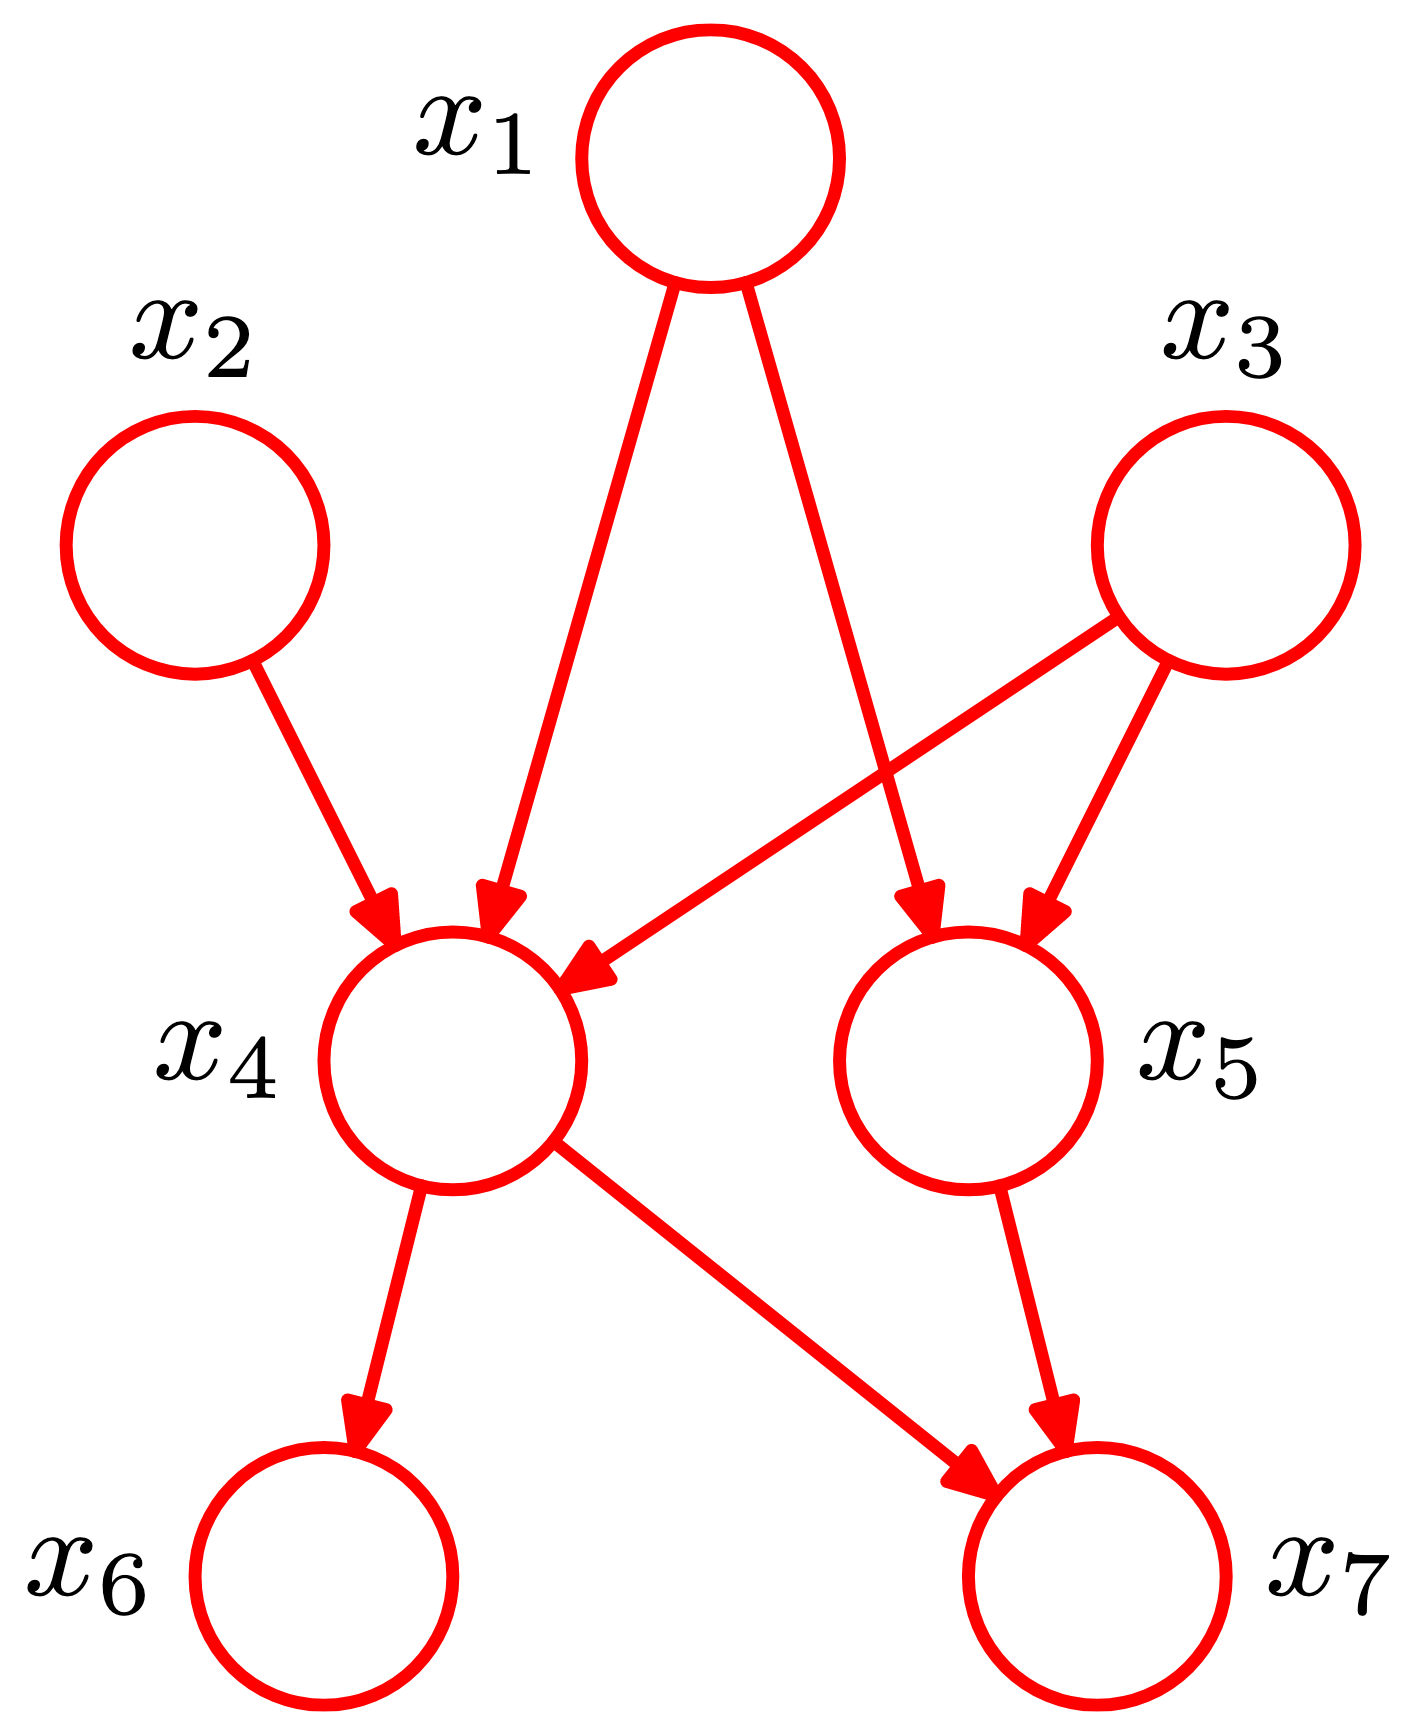
\includegraphics[scale=0.3]{BayesianNetwork1}
	\caption{Example of Bayes Network.}
	\label{fig:BayesianNetwork1}
\end{figure}
The $\mathcal{I}_\ell$ dependency is said to be local (${}_\ell$) since it's defined only wrt to a single variable. \newline
A part from the structure, we need also to have a probability distribution. Let's consider a dataset $\mathcal{D}$ in which all variables are tied with the other by a distribution $p$ which is a joint distribution. We'd like to represent qualitatively with a graph such distribution.\newline
Since the Bayesian Network depends on the independences, it's possible to create a set $\mathcal{I}(p)$ of these by looking at the distribution $p$.\newline
$\mathcal{G}$ is an \textit{independency map} (\textbf{I-map}) for $p$ if $p$ satisfies the local independencies in $\mathcal{G}$:
\[
	\mathcal{I}_\ell(\mathcal{G})\subseteq\mathcal{I}(p)
\]
The sufficient condition for $\mathcal{G}$ to be valid is that all the independences are also in $p$, while the opposite is not always true. Indeed, if some independence from $p$ cannot be modelled into $\mathcal{G}$ via qualitative definition, then they must be modelled quantitatively. \newline
Now we can describe $p$ in terms of the graphical model, that is we can \textbf{factorize} the distribution based on the structure of the model.
\begin{theorem}
$p$ is said to factorize according to $\mathcal{G}$ if:
\begin{equation}
	p(x_1,\hdots,x_m)=\Prod_{i=1}^mp(x_i\vert Parents_{x_i})
	\label{eq:BayesianNetworkFactorization}
\end{equation}
\label{theo:BayesianNetworkFactorization}
\end{theorem}
Mind that this is a double implication: if $\mathcal{G}$ is an I-map for $p$, then $p$ factorizes according to $\mathcal{G}$, then it's true also that if $p$ factorizes according to $\mathcal{G}$, then $\mathcal{G}$ is an I-map for $p$. 
This can be proven as follows.
\begin{proof}
\textit{I-map$\Rightarrow$ factorization}\newline 
If $\mathcal{G}$ is an I-map for $p$, then $p$ satisfies at least these local independences:
\[
\{\forall i~x_i\perp \ND_{x_i}\vert Parents_{x_i} \}
\]
It's possible to order the variable in a topological order relative to $\mathcal{G}$, i.e.:
\[
x_i\rightarrow x_j\Rightarrow i<j
\]
That is the parents have a lower id than the children. Let us now decompose the joint probability using the chain rule as:
\[
p(x_1,\hdots,x_m)=\Prod_{i=1}^mp(x_i\vert x_1,\hdots ,x_{i-1})
\]
Finally local independences imply that for each $x_i$:
\[
p(x_i\vert x_1,\hdots, x_{i-1})=p(x_i\vert Parents_{x_i})
\]
Which by substitution:
\[
p(x_1,\hdots,x_m)=\Prod_{i=1}^m p(x_i\vert Parents_{x_i})
\]
\end{proof}
\noindent Now we need to prove the inverse:
\begin{proof}
Factorization$\Rightarrow$ I-map\newline
If $p$ factorizes according to $\mathcal{G}$, the joint probability can be written as 
\[
p(x_1,\hdots,x_m)=\Prod_{i=1}^mp(x_i\vert Parents_{x_i})
\]
Said $\mathcal{X}$ the set of all variables $x_i$: $\mathcal{X}=\{x_1,\hdots,x_m\}$, let's consider variable $x_m$ (repeat the following steps for the other variable), it's possible to write by the product and sum rules:
\[
p(x_i\vert x_1,\hdots,x_{m-1})=\cfrac{p(x_1,\hdots,x_{m})}{p(x_1,\hdots,x_{m-1})}=\cfrac{p(x_1,\hdots,x_{m})}{\Sum_{x_m}p(x_1,\hdots,x_{m})}
\]
Applying factorisation and isolating the only term containing $x_m$ we get:
\[
	p(x_i\vert x_1,\hdots,x_{m-1})=\cfrac{\Prod_{i=1}^mp(x_i\vert Parents_{x_i})}{\Sum_{x_m}\Prod_{i=1}^mp(x_i\vert Parents_{x_i})}=
\]
\[
	=\cfrac{p(x_m\vert Parents_{x_m})\cancel{\Prod_{i=1}^{m-1}p(x_i\vert Parents_{x_i})}}{\cancel{\Prod_{i=1}^{m-1}p(x_i\vert Parents_{x_i})} \cancel{\Sum_{x_m}p(x_m\vert Parents_{x_m})}}
\]
The sum cancels out because summing all the value of a variable equals to 1. \newline
Hence:
\[
	p(x_i\vert x_1,\hdots,x_{m-1})=p(x_m\vert Parents_{x_m})
\]
\end{proof}
\noindent For example consider Figure~\ref{fig:BayesianNetwork1}. It's possible to write:
\[
	p(x_1,\hdots x_7)=p(x_1)p(x_2)p(x_3)p(x_4\vert x_1,x_2,x_3)p(x_5\vert x_2,x_3)p(x_6\vert x_4)p(x_7\vert x_4,x_5)
\]
Mind that the joint probability $p(x_1, \hdots, x_7)$ is largely influenced by the probability of node 4: $p(x_4\vert x_1, x_2, x_3)$. Now let's suppose that each variable defined a simple binary value, then the total number of possibility would be $2^7$, against the $2^4$ we found right now. This allows to be able to work with a lot of variables. \newline
\begin{definition}[Bayesian Network]
A Bayesian Network is a pair $(\mathcal{G}, p)$ where $p$ factorizes over $\mathcal{G}$ and its represents as a set of conditional probability distribution associated with the nodes of $\mathcal{G}$
\end{definition}
%
%
\subsection{Example}%TODO non so a cosa serva questo esempio
Let's consider another example: genes A and B have independent prior probabilities and gene C can be enhanced by both A and B, with the following probability tables:
\begin{center}
	\begin{tabular}{c|c|cp{2cm}c|c|c}
		Gene&Value&$P(value)$&&Gene&Value&$P(value)$\\
		\cline{1-3}\cline{5-7}
		A&Active&0.3&&B&Active&0.3\\
		A&Inactive&0.7&&B&Inactive&0.7\\
	\end{tabular}
\end{center}
\begin{table}[!h]
	\centering
	\begin{tabular}{cc|cc|cc}
		\multicolumn{2}{c|}{}&\multicolumn{4}{c}{A}\\
		\multicolumn{2}{c|}{}&\multicolumn{2}{c}{Active}&\multicolumn{2}{c}{Inactive}\\
		\hline
		\multicolumn{2}{c|}{}&\multicolumn{2}{c|}{B}&\multicolumn{2}{c}{B}\\
		\multicolumn{2}{c|}{}&Active&Inactive&Active&Inactive\\
		\hline
		C&Active&0.9&0.6&0.7&0.1\\
		C&Inactive&0.1&0.4&0.3&0.9
	\end{tabular}
	\caption{Table showing $p(A,B,\vert C)$.}
\end{table}
%
%
\subsection{Conditional Independence}
First of let's recall Definition~\ref{def:Independence}: two variables $a,b$ are said to be independent written $a\perp b\vert\emptyset$ if: 
\[
p(a,b)=p(a)p(b)
\]
\begin{definition}[Conditional Independence]
Two variables $a,b$ are conditionally independent given $c$, written $a\perp b\vert c$ if:
\[
p(a,b\vert c)=p(a\vert c)p(b\vert c)
\]
\end{definition}
Graphical models allow to directly verify them through the \textbf{d-separation} criterion.
%
%
%
\section{D-separation}
Looking at some simpler graphs, some dependency rules can be inferred and then used on larger graphs by applying them to subgraphs.
%
%
\subsection{Two Nodes}
Given two nodes, or they are independent, hence they are not connected, or they are dependent, hence they are connected.
%
%
\subsection{Three Nodes}
%
\subsubsection{Tail-To-Tail}
Also known as \textit{common cause}.
\begin{center}
	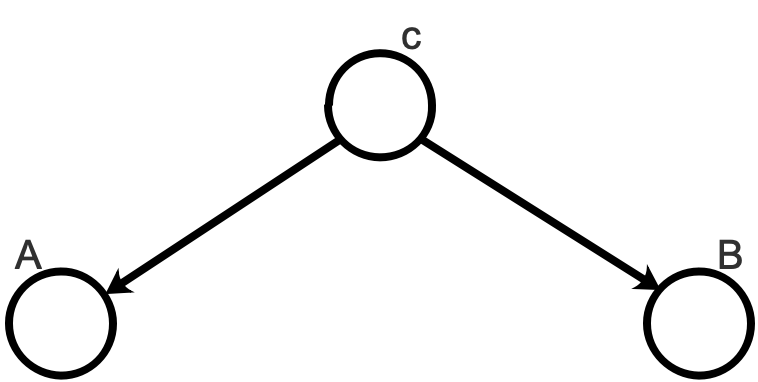
\includegraphics[width=0.4\linewidth]{tailToTailNoGiven}
\end{center}
As for the factorization Equation~\ref{eq:BayesianNetworkFactorization}, the joint distribution can be expressed as:
\[
	p(a,b,c)=p(a\vert c)p(b\vert c)p(c)
\]
The tail-to-tail case says that $a$ and $b$ are \textit{not independent}, written $a \not\!\perp\!\!\!\perp b$. %$a\downmodels b\vert\emptyset$
If $c$ is not given then we have that:
\[
	p(a,b)=\Sum_cp(a\vert c)p(b\vert c)p(c)\neq p(a)p(b)
\] 
On the contrary, if $c$ is given, then they are \textit{conditionally independent}:
\[
p(a,b\vert c)=\cfrac{p(a,b,c)}{p(c)}=p(a\vert c)p(b\vert c)
\] 
\begin{center}
	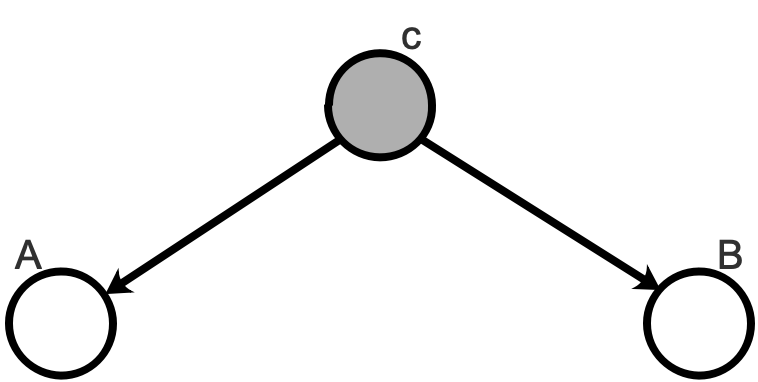
\includegraphics[width=0.4\linewidth]{tailToTailGiven}
\end{center}
Let's consider an example: a company needs to choose the most intelligent ($I$) student between more students. For each student the variables grade $(G)$ and score ($S$) are given. The following graph can be drawn since if the student is intelligent, then it should be seen in both grades and scores. \newline
\begin{minipage}[htp]{\linewidth}
	\begin{minipage}[t]{0.48\linewidth}
		\begin{center}
			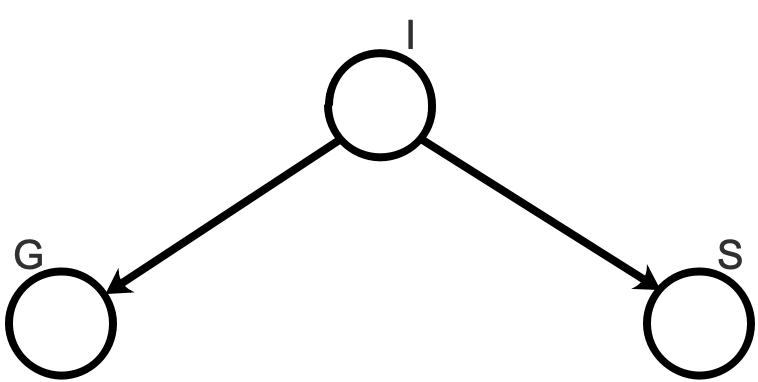
\includegraphics[width=0.7\linewidth]{tailToTailExample1}
		\end{center}
		$G$ and $S$ are directly correlated, for example observing high scores could be indication of having a higher intelligence and hence also higher grades. 
	\end{minipage}
	\hspace{0.04\linewidth}
	\begin{minipage}[t]{0.48\linewidth}
		\begin{center}
			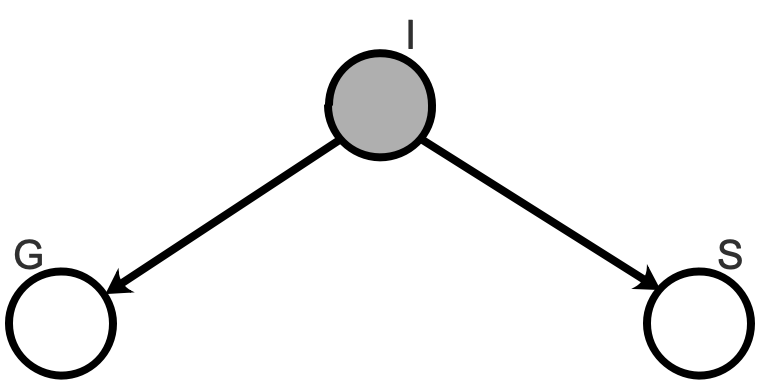
\includegraphics[width=0.7\linewidth]{tailToTailExample2}
		\end{center}
		$G$ and $S$ are not directly dependent since once intelligence has been observed, the correlation disappear and nor $G$ gives more information $S$, nor $S$ gives more information about $G$ than the what we already know. 
	\end{minipage}
\end{minipage}
%
\subsubsection{Head-To-Tail}
Also known as \textit{indirect causal effect}.
\begin{center}
	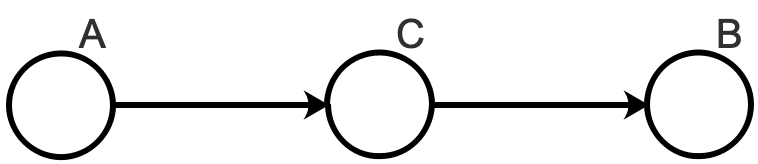
\includegraphics[width=0.4\linewidth]{HeadToTailNoGiven}
\end{center}
The joint distribution can be expressed as:
\[
p(a,b,c)=p(b\vert c)p(c\vert a)p(a)=p(b\vert c)p(a\vert c)p(c)
\]
If $c$ is not given, then then $a$ and $b$ are \textit{not independent}:
\[
p(a,b)=p(a)\Sum_cp(b\vert c)p(c\vert a)\neq p(a)p(b)
\]
If instead $c$ is given, then $a$ and $b$ are conditionally independent:
\[
p(a,b\vert c)=\cfrac{p(b\vert c)p(a\vert c)p(c)}{p(c)}=p(b\vert c)p(a\vert c)
\]
\begin{center}
  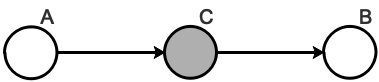
\includegraphics[width=0.4\linewidth]{HeadToTailGiven}
\end{center}
As before, let's consider the example of the intelligence of a student. \newline
\begin{minipage}[htp]{\linewidth}
	\begin{minipage}[t]{0.48\linewidth}
		\begin{center}
			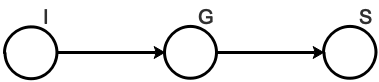
\includegraphics[width=0.7\linewidth]{HeadToTailExample1}
		\end{center}
    Intuitivly, if we observe that the student is intelligent, then we are more inclined to believe that it's grades $G$ are good and that they will have a better score at the interview $S$, that is the probability of these latter events is higher conditioned on the observation that the student is intelligent. 	
	\end{minipage}
	\hspace{0.04\linewidth}
	\begin{minipage}[t]{0.48\linewidth}
		\begin{center}
			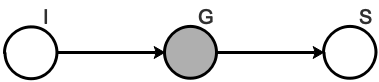
\includegraphics[width=0.7\linewidth]{HeadToTailExample2}
		\end{center}
    Instead if we assume that $G$ is observed, then it's intelligence no longer influences the score of the interview.
	\end{minipage}
\end{minipage}
%
\subsubsection{Head-To-Head}
Also known as \textit{common effect}.
\begin{center}
	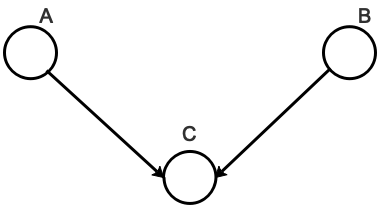
\includegraphics[width=0.4\linewidth]{HeadToHeadNoGiven}  
\end{center}
The joint distribution can be expressed as:
\[
  p(a,b,c)=p(c\vert a, b)p(a)p(b)
\]
If $c$ is not given, then then $a$ and $b$ are \textit{independent}:
\[
  p(a,b)=\Sum_cp(c\vert a, b)p(a)p(b)=p(a)p(b)
\]
If instead $c$ is given, then $a$ and $b$ are not conditionally independent, hence they are conditionally dependent:
\[
p(a,b\vert c)=\cfrac{p(c\vert a,b)p(a)p(b)}{p(c)}\neq p(a\vert c)p(b\vert c)
\]
\begin{center}
  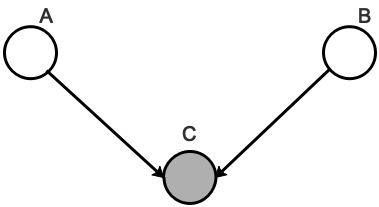
\includegraphics[width=0.4\linewidth]{HeadToHeadGiven}
\end{center}
Let's consider one last time the example of the student that is to be hired from a company. We have said that if $c$ is not given, then $a$ and $b$ are independent, while if $c$ is given they are dependent. Indeed, if $c$ was the score of a test, then the student ($G$) and it was low, we could think that they are actually not that smart, but then if we were to observe that the test was difficult, then we could think that actually they are not \textit{not} intelligent. Hence, $a$ and $b$ are actually correlated if $c$ is given. 
\begin{center}
  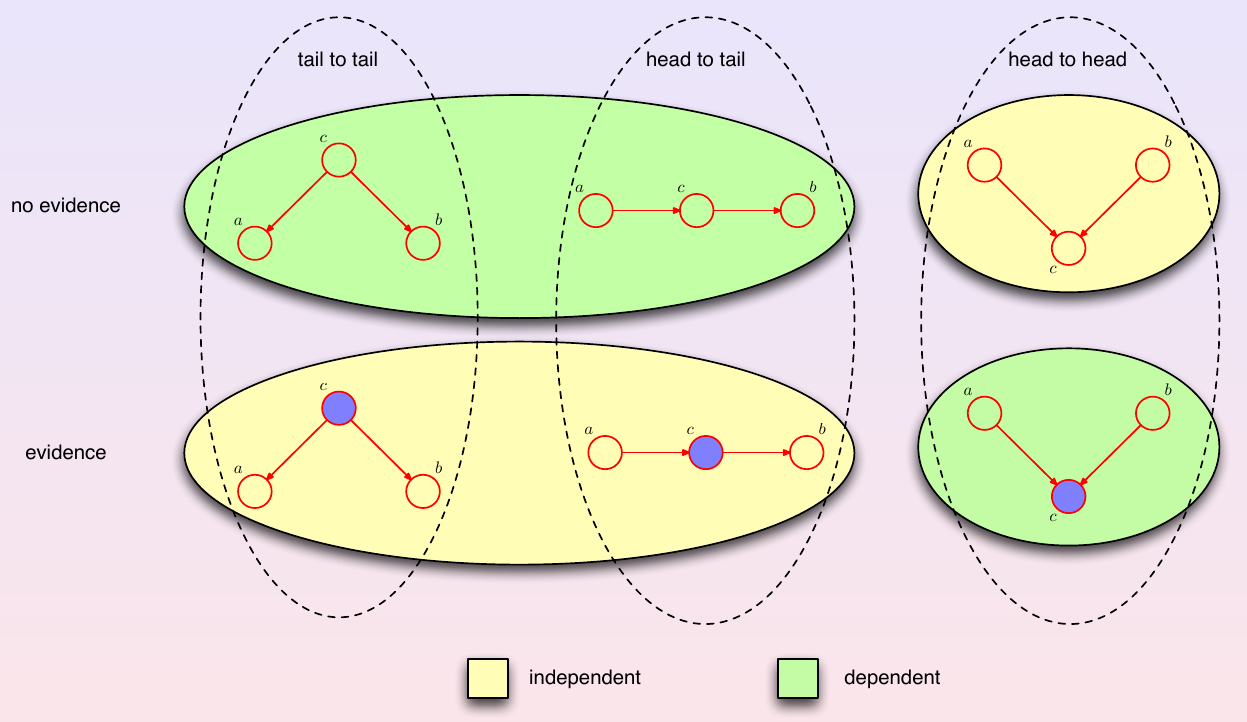
\includegraphics[width=0.8\linewidth]{DSeparationRecap}
\end{center}
\myparagraph{Example Head-To-Head Example}
Let's consider a fuel system of a car. The fuel system is make of:
\begin{itemize}
  \item Battery $B$: can either be charged ($B=1$) or flat ($B=0$);
  \item Fuel tank $F$: can either be full ($F=1$) or empy ($F=0$);
  \item Electric fuel gauge $G$: either full ($G=1$) or empty ($G=0$).
\end{itemize}
Let's now say that the probability of the battery to be charged is $P(B=1)=0.9$ and the probability for the fuel tank to be full is $P(F=1)=0.9$. \newline
Since he electric fuel gauge is conditioned on both:
\begin{center}
  \includegraphics[width=0.8\linewidth]{FuelTankExample1}
\end{center}
we can derive:
\[
  \begin{array}{ll}
    P(G=1\vert B=1,F=1)=0.8&P(G=1\vert B=1,F=0)=0.2\\
    P(G=1\vert B=0,F=1)=0.2&P(G=1\vert B=0,F=0)=0.1\\
  \end{array}
\]


\data{17/10/2019}
$P(F=0\vert G=0)$ non è direttamente presente nelle tabelle e quindi bisogna riuscire a ricrearla.\newline
Per esempio abbiamo una probabilità: $P(G=0\vert F=0)$ e quindi possiamo usare Bayes per girarla:
\begin{center}
	$\displaystyle P(F=0\vert G=0)=\frac{P(G=0\vert F=0)P(F=0)}{P(G=0)}$
\end{center}
Di questo conosimamo solo P(F=0), tutto il resto ce lo calcoliamo:
\begin{center}
	$\displaystyle P(G=0\vert F=0)= \Sum_{B \in \{0,1\}} P(G=0, \vert F=0) =
					\Sum_{B \in\{0,1\}}P(G=0\vert B,F=0)P(B\vert F=0)$
\end{center}
La prima probabilità la abbiamo, la seconda non l'abbiamo, però nella struttura dell'esempio B e $F$ sono indipendenti e quindi $P(B\vert F=0)=P(B)$. quindi otteniamo:
\begin{center}
	$\displaystyle =P(G=0\vert B=0, F=0)P(B=0)+P(G=0\vert B=1, F=0)P(B=1)$
\end{center}
Ora queste probabilità le conosciamo quindi:
\begin{center}
	$\displaystyle =0.9+0.1+(1-0.2)+0.9$
\end{center}
Attenzione che se osserviamo solo B e F i due sono indipendenti, se invece consideriamo tutta la rete, allora abbiamo G e B e F sono dipendenti. Mind that also saying given doesn't mean we know the value for sure, it just means we assume it gets that value. \newline
Dobbiamo ora calcolarci $P(G=0)$. 
\begin{center}
	$\displaystyle P(G=0)=\Sum_{F,B}P(G=0, F, B)=\Sum_{F,B}P(G=0\vert F, B)P(F)P(B)$
\end{center}
Di queste probabilità abbiamo tutti i dati quindi possiamo concludere.\newline
\section{d-separation}
Abbiamo visto le 3 diverse strutte nel caso di 3 nodi. Consider tail to tail and for example earthquake->alarm, burglar->alarm if you see the alarm you can think of the burglar, but if you see earthquake, than for sure it's not a burglar, so the two fathers are related. \newline
If we add a fourth node phone call from alarm, then
\subsection{Definition}
Consideriamo un grafo come quello in figura. Vogliamo fare dei calcoli arbitrari sulla dipendenza, per esempio che A=x1, x2 sono indiependenti da B=x5 e x7 e un altro set $C=\emptyset$. Possiamo usare le regole che abbiamo visto adesso. Praticamente per ogni nodo in un set dobbiamo vedere tutti i possibbili percorsi che ci portano a un altro set e sfruttando le regole di prima possiamo dire che non esiste un passo se ad esempio abbiamo tail to tail o head to tail con evidence nel mezzo, oppure head to head senza evidence. So x4->x6 is head to tail, non ho informazione quindi è libero, x4,x5,x6 è head to head e non c'è evidence quindi è bloccato. Consideriamo il percorso x1x4x6x7, i primi 3 sono head to tail senza evidence quindi posso passare, e anche dopo x4x6x7. \newline
Supponiao ora che $C$ contenga x6, allora il path 3 è bloccato, mentre il path 1 non è più bloccato perchè x6 diventa evidence.\newline
$C$ quindi è il set con l'evidence. 
\section{BN independences}
Abbiamo visto le indipendenze locali, ossia indiepndenze dei nodi rispetto a tutto il resto. A questo si aggiungono indipendenze globali (che racchiudono anche le primme), definire come in slide. \newline
\section{Equivalence classes}
Possiamo raggruppare le indipendenze in classi, ad esempio head-to-head in una direzione o nell'altra producono la stessa cosa, come anche tail to tail nel caso senza evidence. Due strutture sono nella stessa classe si equivalenza se codificano la stessa dipendenza. In principio ogni struttura da una classe è equivalente per rappresentare i dati. \newline
\section{l-maps}
Per riuscire ad avere un buon modello bisogna riuscire a codificareil amggior numero di strutture, quindi abbbiamo una definizone di mappa minima come quella in slide. Questo non soddisfa il fatto che riusciamo a prendere tutte le dipendenze. \newline
Al contrario una mappa perfetta è una mappa che riesce a prendere tutte le dipendenze. Ovviamente una mappa perfetta è anche minima, ma non viceversa. Esiste un algoritmo per trovare una mappa perfetta per una distribuzione ed è esponenziale rispetto al numero di connessioni massime che un nodo ha. Ci sono della distribuzione che non hanno delle mappe perfette, per risolvere queste distribuzioni si usano dei grafi non diretti chiamati Markov Networks. \newline
\section{Making bayesian networks}
Un esperto deve fornirci le variabili di interesse, ad esempio i sintomi e quello che potremmo voler trovare. A questo punto vogliamo costruire dei collegamenti e per fare questo vogliamo collegare varaibili che sono in relazione causale, questo ci permette di avere anche un grafo con meno collegamenti. A questo punto dobbiamo mettere le probabilità per ogni configurazione. \newline
Quello che si fa di solito è prendere un sacco di dati e imparare i parametri e in alcuni casi anche la struttura (partendo comunque da una struttura minima).
\section{Inference in graphical model}
Un BN, come tutti i cosi grafici, modella una probabilità congiunta. Per questo motivo si ha:
\begin{center}
	$\displaystyle P(X\vert E=e)=\frac{p(X,E=e)}{P(E=e)}$
\end{center}
Vedi fogli \ins(6) ma è troppo grande, quindi possiamo usare la scomposizione. La struttura più semplice che possiamo pensare è una catena dove ogni varaibile ha una connessione a quella dopo. In questo modo la probabilità di tutte le variabili nella reteè:
\begin{center}
	$\displaystyle P(X)=P(x1)P(X2\vert x1)...P(x_{N}\vert x_{N-1})$
\end{center}
Supponiamo di voler calcolare la probailità di una variabile senza condizione:
\begin{center}
	$\displaystyle P(x_n)=\sum_{x_1}...\Sum_{x_N}P(X)$
\end{center}
In questo modo ad esempio $\Sum_{x_N}$ è solo la parte finale della formula di prima e tutto il resto invece è costante:
\begin{center}
	$\displaystyle \mu_\beta(x_{n-1})=\Sum_{x_N}P(x_N\vert x_{N-1})$
\end{center}
Se ora si sommano tutti i valori si ottiene 1, ma non sempre??????\newline
Possiamo rsicrivere come: 
\begin{center}
	$\displaystyle \sum_{x_1}...\Sum_{x_{N-1}}P(x_1)P(x_2\vert x_1)...P(x_{n-1}\vert x_{n-2})\mu_\beta(x_{n-1})$
\end{center}
A questo punto consideriamo la sommatoria per $n-1$ ed è la stessa cosa, tutto costante tranne l'ultima cosa:
\begin{center}
	$\displaystyle \mu_\beta(x_{n-2})=\Sum$
\end{center}
E continuo fino ad arrivare da qualche parte e si ha:
\begin{center}
	$\displaystyle \mu_\beta(x_n)=\Sum_{x_{n+1}}P(x_{n+1}\vert x_n)\mu_\beta(x_{n+1})$
\end{center}
Ora manca qualche altra sommatora, cioè non ci si capisce più niente e andadno al contrario si ha:
\begin{center}
	$\displaystyle \mu_\alpha(x_2)=\Sum_{x_1}P(x_1)P(x_2\vert x_1)$\\
	$\displaystyle \mu_\alpha(x_3)=\Sum_{x_2}P(x_3\vert x_2)\mu_\alpha(x_2)$
\end{center}
E alla fine si ha mettendo tutto insieme che:
\begin{center}
	$\displaystyle p(X_n)=\mu_\alpha(X_n)\mu_\beta(X_n)$
\end{center}
Migliorando le prestazioni per qualche altro motivo portandole da esponenziali a qualcos'altro.\newline 
Possiamo pensare a $\mu$ come un messaggio e mandarlo avanti $\alpha$ o indietro (backwards) $\beta$.\newline
Supponiamo di avere fatto tutti i calcoli e mandati i messaggi e abbbiamo la nostra rete e dobbiamo computare $X_{n+1}$ quindi dovremmo ricominciare a mandare tutti i messaggi, ma la maggior parte sono li stessi quindi non vogliamo ricalcolarli. Al posto di fare questo si manda un messaggio dall'inizio alla fine e dalla fine all'inizio e boh. \newline
Questo è tutto senza evidence, ma di solito abbiamo anche questa. Dobbiamo quindi modiifcare l'algoritmo per tenere conto dell'evidence: abbiamo calcolato $P(x_n)$.\newline
Questo funziona con le catene, ma non sono l'unico tipo di struttura. altri tipo di struttura sono gli alberi ossia strutture dove ogni nodo ha un solo genitore, uno che non ha padri che è la radice e nodi che non hanno figli che sono le foglie, oppure poly-tree: si ha comunque un solo percorso tra coppie di nodi. Anche gli undirected trees, questo perchè l'inferenza che abbiamo visto prima è valida sia per BN che per Markov Networks. 
\section{Factor graph}
Il modo per parlare di queste strutture da catenre è passare per una struttura intermedia chiamata factor graph utile solo per fare gli inference graph. \newline
Questo grafo ha un nodo per ogni variabbile e anche nodi (detti factor nodes) per ogni evidence (forse= che ha. È anche un grafo non direzionale. \newline
Ogni nodo factor deve essere collegato a tutti i nodi delle probabilità da cui deriva la scomposizione. 
